\documentclass[a4paper,12pt,twoside]{article}%twoside
\usepackage[utf8]{inputenc}
\usepackage[dutch]{babel}
\usepackage{fancyhdr, amsmath, color, graphicx, enumitem, tabularx, hyperref, longtable, multirow, placeins, apacite, subcaption,marvosym,multicol}
\usepackage[framemethod=tikz]{mdframed}
 
  \usepackage[margin=2.5cm,headheight=68pt]{geometry}
 %\usepackage[total={16cm, 22cm}]{geometry}
 
\pagestyle{fancy}
\fancyhf{}
\fancyhead[LE,RO]{Specifieke Lerarenopleiding voor CVO-studenten}%'E': even page, 'O': odd page
\fancyhead[RE,LO]{Didactische Competentie Stage}
\fancyfoot[RE,CO]{}
\fancyfoot[LE,RO]{KU Leuven campus Kortrijk Kulak   \thepage}
%\renewcommand{\labelitemi}{$\circ$}
 
\definecolor{CVO}{RGB}{232, 0, 97}
\setlength\parindent{0pt}
\title{Stageportfolio}
\author{Kevin Truyaert}
\date{}
 
 
 % %FOOTER IN MDFRAMED
 \usepackage{footnote} 
 \newenvironment{mdframedwithfoot}
 {   
     \savenotes
     \begin{mdframed}
     \stepcounter{footnote}
     \renewcommand{\thefootnote}{\arabic{footnote}}
     }
 {
     \end{mdframed}
     \spewnotes
 }
 
 
 %FOOTER IN PARBOX
 \makeatletter
 \newcommand{\global@insert}[2]% #1=box number, #2=vertical list
 {\bgroup
   \setbox\@tempboxa=\box#1
   \global\setbox#1=\vbox{\unvbox\@tempboxa #2}
 \egroup}
 
 \long\def\@footnotetext#1{\global@insert\footins{%
  \reset@font\footnotesize
  \interlinepenalty\interfootnotelinepenalty
  \splittopskip\footnotesep
  \splitmaxdepth \dp\strutbox \floatingpenalty \@MM
  \hsize\columnwidth \@parboxrestore
  \protected@edef\@currentlabel{%
  \csname p@footnote\endcsname\@thefnmark
  }%
  \color@begingroup
  \@makefntext{%
  \rule\z@\footnotesep\ignorespaces#1\@finalstrut\strutbox}%
  \color@endgroup}}%
 \makeatother
 %%%%%%%%%%%%%%%%%%%%%%%%%
 
 %Strikeout and highlight text
  \usepackage{soul}
  \usepackage{tikz} % only to get \foreach
  
  %\definecolor{yellow}{RGB}{255,255,0}
  \sethlcolor{yellow}

 % \newcommand*{\YellowHighlight}[1]{{\hl{~#1~}}}
  \newcommand*{\PinkHighlight}[2]{{\hspace{-1.5mm}\colorbox{pink}{\parbox{#2}{~#1~}}}}
  \newcommand*{\GreenHighlight}[2]{{\hspace{-1.5mm}\colorbox{green}{\parbox{#2}{~#1~}}}}
  \newcommand*{\YellowHighlight}[2]{{\hspace{-1.5mm}\colorbox{yellow}{\parbox{#2}{~#1~}}}}
  % % % % % %
  
  \usepackage{tabularx,pdflscape,pdfpages}
  
  \newcolumntype{C}[1]{>{\centering\let\newline\\\arraybackslash\hspace{0pt}}m{#1}}
 
 \begin{document}
\maketitle


\section*{Identificatiegegevens}
\begin{center}
	\begin{tabular}{ll}
	\hline
	Naam: & Kevin Truyaert\\ \hline
	Adres: & Bolle-Akkerweg 4\\
		& 8800 Roeselare\\\hline
	Telefoon: & 0032495/928460\\\hline
	Mail: & kevin.truyaert@student.kuleuven.be\\\hline
	Naam stagebegeleider: & Cato De Baets\\ \hline
\end{tabular}
\end{center}

\newpage
\tableofcontents
\newpage


% !TeX root = Stageportfolio.tex

\begin{landscape}
\section{Observatie- en stageplanning}

\subsection{Observatieplanning}

\begin{tabularx}{1.56\textwidth}{|C{0.15\textwidth}|C{0.14\textwidth}|C{0.14\textwidth}|C{0.1\textwidth}|C{0.1\textwidth}|C{0.05\textwidth}|C{0.35\textwidth}|X|}
	
	
\end{tabularx}
	

\subsection{Actieve stage}
\begin{table}[]
	\begin{tabularx}{1.56\textwidth}{|X|}
		\hline
		Naam stagair:  Kevin Truyaert  \\
		Tel.: 0495/928460 \hspace{3cm} e-mail: kevin.truyaert@student.kuleuven.be  \\
		Naam en adres opleidingsinstituut:  KU Leuven Campus Kulak Kortrijk, Etienne-Sabbelaan 53, 8800 Kortrijk  \\
		Naam directie: \\
		Naam stagecoördinator:  David Dudal \\
		\hline
	\end{tabularx}
\end{table}
		
	\begin{tabularx}{1.56\textwidth}{|C{0.15\textwidth}|C{0.14\textwidth}|C{0.14\textwidth}|C{0.1\textwidth}|C{0.1\textwidth}|C{0.05\textwidth}|C{0.35\textwidth}|X|}
		\hline
		\textbf{Datum} & \textbf{Vestiging} & \textbf{\begin{tabular}[C]{@{}l@{}}Aantal\\ stage-uren\end{tabular}} & \textbf{\begin{tabular}[C]{@{}l@{}}Uur \end{tabular}}    & \textbf{Lokaal}& \textbf{\begin{tabular}[C]{@{}l@{}}AV\\TV\\PV\\KV\end{tabular}}& \textbf{\begin{tabular}[C]{@{}l@{}}Onderwijsvorm\\ graad en lj\\ Vak en lesonderwerp\end{tabular}}  &  \textbf{\begin{tabular}[C]{@{}l@{}}Naam vakmentor\\ + handtekening\end{tabular} } \\ \hline
		27/11/2019 & Kulak & 1-3 & 10:30-13:00 & A352 & AV & Universiteit\newline 2e jaar Handelsingenieur\newline Conceptuele natuurkunde\newline werkzitting elektromagnetisme & \\ \hline
		4/12/2019 & Kulak & 4-6 & 10:30-13:00 & A352 & AV & Universiteit\newline 2e jaar Handelsingenieur\newline Conceptuele natuurkunde\newline werkzitting elektromagnetisme & \\ \hline
		11/12/2019 & Kulak & 7-9 & 10:30-13:00 & A352 & AV & Universiteit\newline 2e jaar Handelsingenieur\newline Conceptuele natuurkunde\newline werkzitting elektromagnetisme & \\ \hline
	\end{tabularx}
\begin{tabularx}{1.56\textwidth}{|C{0.15\textwidth}|C{0.14\textwidth}|C{0.14\textwidth}|C{0.1\textwidth}|C{0.1\textwidth}|C{0.05\textwidth}|C{0.35\textwidth}|X|}
	\hline
		18/12/2019 & Kulak & 10-12 & 10:30-13:00 & A352 & AV & Universiteit\newline 2e jaar Handelsingenieur\newline Conceptuele natuurkunde\newline werkzitting elektromagnetisme & \\ \hline
		 &  &  &  &  &  &  & \\ \hline
	\end{tabularx}
		


		
\end{landscape}		
		




% !TeX root = Stageportfolio.tex

\section{Persoonlijk ontwikkelingsplan}
\begin{tabularx}{\textwidth}{|p{0.15\textwidth}|p{0.795\textwidth}|}
	\hline
	\textbf{Lesdoel 1} & 
	\underline{FG 1: de leraar als begeleider van leer- en}\newline \underline{ontwikkelingsprocessen}\newline
	
	1.8 De leraar kan observatie en evaluatie voorbereiden en uitvoeren met het oog op bijsturing en remediëring als onderdeel van het leerproces van een lerende(n) en kan die observatie-en evaluatiegegevens gebruiken om zijn eigen didactische handelen in vraag te stellen en bij te sturen waar nodig.\\ \hline
	Actie 1 & Tijdens het lesgeven wil ik veel in interactie treden. Dit zou ik met zoveel mogelijk leerlingen willen doen en niet steeds dezelfde leerlingen aan bod laten komen. Het lijkt mij uitdagend om dit in realiteit om te zetten. Door hen gerichte vragen te stellen, kan ik kijken waar er mogelijke problemen zijn met de leerstof en van daaruit werken om de lesdoelen begrijpelijk te maken voor alle leerlingen. \\ \hline
	Actie 2 & Na het verbeteren van een taak, een toets of extra oefeningen wil ik die met de leerling(en) overlopen door de meest voorkomende fouten te bespreken. Zo kan ik hen bijsturen en kan ik de belangrijkste punten aanhalen waar er problemen waren. Tegelijkertijd kom ik zo te weten waar ik te weinig nadruk gelegd heb tijdens de les. Hier kan ik nu mee aan de slag om mijn toekomstige lessen aan te passen en om te verhinderen dat hetzelfde soort fouten bij soortgelijke zaken minder gemaakt worden. \\ \hline
\end{tabularx}


\vspace{0.5cm}
\begin{tabularx}{\textwidth}{|p{0.15\textwidth}|p{0.795\textwidth}|}
	\hline
	\textbf{Lesdoel 2} & \underline{FG3: de leraarals inhoudelijk expert} \newline\newline 3.3 De leraar beheerst de kennis en vaardigheden met betrekking tot de (vak)didactiek van zijn onderwijsopdracht. Hij kan die  actualiseren, verbreden en verdiepen. \\ \hline
	Actie 1 & Ik wil als leraar in staat zijn om de theorie interessant over te kunnen brengen. Dit wil ik doen door actuele zaken als voorbeeld van die theorie te gebruiken. Een voorbeeld hiervan: ieder jaar wordt een flitsmarathon aangekondigd. De flitscamera werkt volgens het Dopplereffect. Dus wanneer ik dat moet uitleggen aan de leerlingen, kan ik de flitscamera als voorbeeld gebruiken. Door actuele thema's en alledaagse voorwerpen te linken met fysische verschijnselen, hoop ik dat de leerlingen de wereld rond hen beter begrijpen. \\ \hline
	Actie 2 & Als leerkracht vind ik het belangrijk dat je de leerstof die je aan het bespreken bent, goed begrijpt en dat je de achtergrond ervan ook kent, ook al behandel je die niet in de les. Ik vind dat je als leerkracht de leerstof enkele niveaus dieper moet beheersen dan dat je ze moet overbrengen. Op die manier kan je beter begrijpen vanwaar alles komt en zou je meerdere invalswegen moeten hebben om de te geven leerstof aan je leerlingen over te brengen. \\ \hline
\end{tabularx}


\vspace{0.5cm}
\begin{tabularx}{\textwidth}{|p{0.15\textwidth}|p{0.795\textwidth}|}
	\hline
	\textbf{Lesdoel 3} & \underline{FG5:  de leraar als innovator - de leraar als onderzoeker}\newline\newline
	5.1 De leraar kan de kwaliteit van zijn onderwijs verder ontwikkelen. De leraar kan zijn eigen onderwijspraktijk en zijn eigen functioneren in vraag stellen en bijsturen (verbeteren) door te innoveren om zijn eigen praktijk te verbeteren.\\ \hline
	Actie 1 & Ik verzorg reeds drie jaar oefenzittingen aan de universiteit. Dit jaar wil ik iets nieuws proberen en de studenten actiever de oefeningen laten maken. Ik wil hen in groep aan de oefeningen laten werken, waardoor ze met elkaar in interactie kunnen treden om de oefeningen samen tot een goed eind te kunnen brengen. Op die manier wil ik tijdens mijn oefenzittingen voor innovatie bij lessen in het hoger onderwijs zorgen. \\ \hline
	Actie 2 & Bij de lessen die ik in het middelbaar zal verzorgen, wil ik terugkoppelen naar mijn stagelessen die ik bij DCO deed. Hier gaf ik telkens de introductieles van een nieuw stuk theorie. Die gaf ik relatief `klassiek', waarbij ik als leerkracht veel aan bod kwam. Ik wil nu proberen om de leerlingen zal actiever aan de slag te zetten bij de start van een nieuw stuk. Ik zie dit nu ook meer zitten, omdat ik meer dan één les(blok) per klas zal brengen. Dit zal als gevolg hebben dat ik een groter plan kan uitwerken en zo proberen om mijn eigen lesgeven te innoveren.    \\ \hline
\end{tabularx}


\begin{landscape}
	
\section{Bespreking lesobservaties}

\begin{tabularx}{1.56\textwidth}{|C{0.25\textwidth}|C{0.1\textwidth}|C{0.25\textwidth}|X|}\hline
	\textbf{Naam student: Kevin Truyaert} & & Aandachtspunten (o.b.v. POP) & Reflectie:\newline -Wat leerde ik uit mijn observatie over mijn aandachtspunten? \newline -Wat doe ik ermee tijdens mijn stage?\\\hline
	Observatieles \newline Datum: & 1 & & \\
	Klas: \newline Lesonderwerp: & 2 & & \\\hline
	Observatieles \newline Datum: & 1 & & \\
	Klas: \newline Lesonderwerp: & 2 & & \\\hline
	
\end{tabularx}
\end{landscape}

% !TeX root = Stageportfolio.tex



\begin{landscape}
	\section{Lesvoorbereidingen en bijhorende media}
	\begin{tabularx}{1.56\textwidth}{|p{0.55\textwidth}|X|}\hline
		\textbf{Administratieve gegevens}\newline\newline
		Kevin Truyaert\newline\newline
		Universiteit\newline
		Handelsingenieur, 2de fase\newline
		Leerplannummer: De inhoud is terug te vinden op de ECTS fiche: \href{https://onderwijsaanbod.kuleuven.be/syllabi/n/D0W55AN.htm}{https://onderwijsaanbod.kuleuven.be/syllabi/n /D0W55AN.htm} \newline
		Lesonderwerp: `Oefenzitting elektromagnetisme: wat zijn de relaties tussen de elektrische kracht, de  elektrische potentiaal, de elektrische flux en de elektrische capaciteit' & \textbf{Doelstellingen}\newline
		\newline\newline 
		\underline{Leerplandoelen}\newline - Elektriciteit: elektrische lading, elektrisch veld (wetten van Coulomb en Gauss), elektrische flux, elektrische potentiaal, energie in een elektrisch veld \newline\newline
		\underline{Lesdoelen}\newline
		\vspace{-0.5cm}
		\begin{enumerate}
			\item De studenten kunnen via de wet van Coulomb de elektrostatische kracht tussen ladingen berekenen.
			\item De studenten kunnen de relatie tussen de elektrostatische kracht, het elektrisch veld en een lading toepassen in een probleem.
			\item De studenten kunnen de elektrostatische kracht binnen de tweede wet van Newton herkennen.
			\item De studenten kunnen een Gaussoppervlak in een situatie opstellen.
			\item De studenten zijn in staat om de elektrische flux te bepalen met gebruik van een Gaussoppervlak.
			\item De studenten kunnen het elektrisch veld en de elektrische flux van een boloppervlak in functie van de afstand afleiden.
			\item De studenten kunnen het elektrisch veld en de elektrische flux van een opgevulde, geleidende bol in functie van de afstand afleiden.
			\item De studenten kunnen.
		\end{enumerate} \\\hline
	\end{tabularx}


	\begin{tabularx}{1.56\textwidth}{|p{0.55\textwidth}|X|}
		\hline
		\multirow{2}{0.55\textwidth}{\textbf{Beginsituatie}\newline De studenten hebben de theorie rond de  begrippen van `Elektrisch veld', `Elektrische potentiaal', `Elektrische flux' en de wet van Coulomb in de week van 12-15 november gezien, twee weken voor de oefenzitting. Hierdoor zullen ze al tijd gehad hebben om de theorie te bekijken, wat aangemoedigd wordt door het maken van een voorbereidende opdracht die ik de week voor de oefenzitting op Toledo plaats.\newline\newline De minderheid van de studenten heeft  interesse bij mechanica, het eerste deel van de cursus, getoond. Het gedeelte over elektromagnetisme ervaren ze meestal interessanter. Er zijn 28 studenten die deze sessie volgen, maar gemiddeld gezien zijn er 25 studenten aanwezig geweest bij de voorbije lessen.\newline\newline Het lokaal kan 30 studenten plaatsen. Er is een dubbel krijtbord ter beschikking en de mogelijkheid tot projectie. Wanneer er geprojecteerd wordt, hangt het projectiescherm grotendeels over beide borden.    }& \textbf{Acties}\newline  - Om de studenten te stimuleren om zelf aan de slag te gaan, wil ik hen in groepjes van vier tot zes studenten aan de slag zetten. Hierdoor kan ik gerichtere feedback geven, aangezien de studenten onderling elkaar kunnen aanzetten tot het vinden van oplossingen. Naast de helpende rol, kan ik ook interacties tussen de studenten onderling volgen en inspringen waar nodig: ofwel bij het maken van een fout, of wanneer ik hun uiteenzetting zeer goed vind en er nog dieper op in wil gaan. Dit wil ik steeds vanuit het onderwijsleergesprek proberen te realiseren.  \newline \\ \cline{2-2}
		  & \textbf{Bronnen}\begin{itemize}
		  	\item Dudal, D., Temmerman, E., Truyaert, K., Heymans, S. (2019). Slides conceptuele natuurkunde
		  	\item Dudal, D., Temmerman, E., Truyaert, K., Heymans, S. (2019). Oefeningenbundel conceptuele natuurkunde
		  	\item Giancoli, D. C. (2008). Physics for scientists and engineers. Pearson Education International.
		  \end{itemize}\\ \hline
	\end{tabularx}


\newpage
	
	
	
	\begin{tabularx}{1.56\textwidth}{|p{1.5cm}|p{6cm}|X|p{4cm}|}
		\hline
		\textbf{Nr. lesdoel } & \textbf{Inhoud (timing)}  & \textbf{Organisatie } & \textbf{Media } \\ \hline
		&\underline{Inhoudelijke titel (timing)}
	    \textcolor{gray}{(Naast een inhoudelijke titel en de timing, noteer je kort en samenvattend de kerninhoud van de lesfase; uitgebreide informatie/oefeningen/… neem je op in de uitgewerkte media [verwijzen!])}
	    &  \textcolor{gray}{(Naast de benaming van de specifieke werkvorm [bv. placemat-oefening/basis-expertengroep/… en dus níet groepswerk], noteer je kernachtig het organisatorisch verloop van de lesfase. Noteer eveneens belangrijke vragen die je wil stellen.) }
		& 
		\\ \hline
	\end{tabularx}
	
	
	
	
	
	
	
	
\end{landscape}







\section{Bespreking meso-activiteiten}
Stel per meso-activiteit een verslag op op basis van volgende criteria:
\begin{itemize}
	\item Korte situering van de drie activiteiten.
 	\item Omschrijving van twee aspecten die je voor jezelf geleerd hebt uit de deelname aan de activiteiten
	\item  Toon aan met twee voorbeelden dat de activiteiten een meerwaarde zijn voor de leerkrachten.
	\item Toon aan met twee voorbeelden dat de activiteiten een meerwaarde vormen voor de leerlingen.
	\item Bespreek hoe het komt dat bepaalde activiteiten geen echte meerwaarde hebben voor leerlingen en op welke manier deze aangepast kunnen worden om toch nog functioneel te zijn voor het leerproces van de leerlingen.
\end{itemize}

\subsection{Omschrijving van de activiteiten}
\subsubsection{Meso-activiteit 1: kinderuniversiteit Kulak}  Op zaterdag 26 oktober ging aan de katholieke universiteit campus kulak kortrijk de kinderuniversiteit door. Tijdens deze dag kunnen jongeren tussen 8 en 13 jaar ofwel de voormiddag, namiddag of hele dag op de universiteit doorbrengen. Per sessie wordt er zowel een lezing (45min) als een workshop (1u30min) aangereikt; de lezing wordt door iedereen gevolgd, waarna de jongeren zich verspreiden om per 20 à 25 een workshop te volgen.\newline


De 15e editie van de kinderuniversiteit stond in het teken van `reis door de tijd'. De werknemers van de Kulak voorzagen tien verschillende workshops. Enkele personen binnen de fysica, waartoe ik behoor, bedachten een workshop genaamd `Bouw nu een telescoop en kijk straks naar het Universum van vroeger!'. Hiermee willen we de leerlingen bekend maken met de werking van lenzen, dat je de kleuren van de regenboog uit wit licht kan halen en dat je in het verleden kijkt wanneer je met een telescoop naar de sterren kijkt. De leerlingen krijgen tijdens de workshop eerst een halfuur uitleg van de professor door middel van een presentatie met slides en demonstratiemateriaal. Tijdens deze presentatie begint de professor met uit te leggen hoe licht werkt. Hij toont breking van licht met behulp van een laserstraal, een glazen halve cirkel (om het licht te breken) en wat krijtstof. Om reflectie duidelijk te maken, wordt er een spiegel aan de leerlingen doorgegeven. Daarna legt de prof uit hoe zowel holle als bolle lenzen werken, hoe ze ervoor zorgen dat dingen vergroot en verkleind worden en hoe je lenzen kan gebruiken om naar de ruimte te kijken. Daarna legt de professor nog uit dat het licht wel heel snel gaat, maar niet oneindig snel. Hierdoor zie je sterren zoals ze in het verleden waren. \newline\newline

Na deze uitleg gaan de leerlingen aan de slag met het maken van een minitelescoop. Hiervoor gebruiken ze:
\begin{itemize}
	\item 2 PVC-buizen met een verschillende diameter die in elkaar schuiven
	\item Twee verschillende lenzen
	\item 3D-geprinte lenshouders
	\item Plakband en versiering.
\end{itemize}
\begin{figure}[!h]
	\centering
	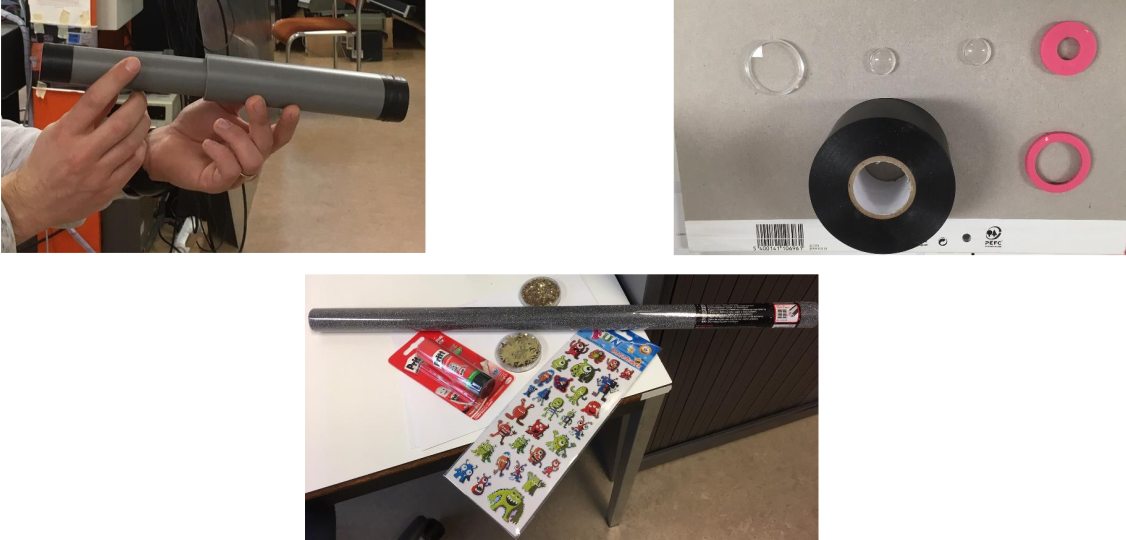
\includegraphics[width=0.9\textwidth]{Telescoop}
	\caption{Het materiaal waarmee de telescoop gemaakt wordt.}
	\label{Fig::Telescoop}
\end{figure}
Tijdens het maken van hun telescoop werden de leerlingen per drie meegenomen om zelf de eigenschappen van lenzen te ondervinden. Er werd een figuur op doorschijnende folie afgedrukt die een hond voorstelt en wanneer je de figuur ondersteboven houdt een kat toont. De figuur staat hieronder in beide opzichten.

\begin{figure}[!b]
	\centering
	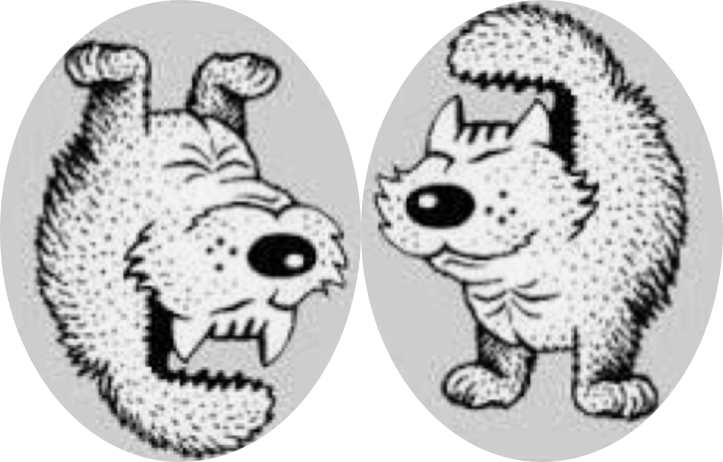
\includegraphics[width=0.5\textwidth]{HondKat}
	\caption{De figuur die gebruikt werd om de  leerlingen de eigenschappen van bolle lenzen te laten ondervinden.}
	\label{Fig::HondKat}
\end{figure}
Door middel van een opstelling met bolle lenzen is het mogelijk om beide figuren zichtbaar te maken, aangezien bolle lenzen het beeld kunnen omdraaien. De opstelling werd aan de leerlingen voorgesteld en iedere component werd benoemd. Door aan de  leerlingen de vraag te stellen hoe het mogelijk is dat beide beelden uit het ene beeld voortkomen wisten er sommigen de eigenschappen van bolle lenzen, die ze net gehoord hadden, te gebruiken om dit te verklaren. 

Wanneer alle jongeren hun telescoop gemaakt hebben, kunnen ze op zoek gaan naar hun naam die op een ster geschreven staat. Die sterren hangen een eindje verder, waardoor hun namen niet zichtbaar zijn met het blote oog. 

\subsection{Twee aspecten die ik voor mezelf geleerd heb}

\subsection{Twee voorbeelden die aantonen dat de activiteiten een meerwaarde zijn voor leerkrachten}

\subsection{Twee voorbeelden die aantonen dat de activiteiten een meerwaarde zijn voor leerlingen}


\subsection{Voorbeelden die geen echte meerwaarde hebben voor de  leerlingen en op welke manier deze aangepast kunnen worden om toch nog functioneel te zijn voor het leerproces van de leerlingen}






\section{Evaluatiedocumenten vakmentor}

\section{Evaluatie document klasbezoek stagebegeleider}

\section{Eindreflectie}
Stel een eindreflectie op waarin je volgende aspecten behandelt: 

1) Waren er factoren die bevorderend of belemmerend werkten m.b.t. het goed doorlopen van je stage? 
2) Waarvoor had je graag bijkomende begeleiding gekregen van je vakmentoren? 
3) Waarvoor had je graag bijkomende begeleiding gekregen van je stagebegeleider? 
4) Bekijk aandachtig de acties die je in het begin van je stage opstelde in jouw POP . Ga na of je via de acties jouw leerdoelen hebt behaald. Verwijs heel duidelijk naar informatie in je portfolio waar en hoe je deze acties aan bod liet komen. 
5)  Bestudeer nogmaals het opleidingsprofiel en de basiscompetenties van een leraar (link):  bespreek minstens 5 basiscompetenties die je succesvol hebt behaald tijdens het uitvoeren van je stage. 
Jouw eindreflectie is maximaal drie A4-pagina’s lang. 



\section{Voorbereiding eindassessment}

Om het eindassessment voor te bereiden, kan je gebruik maken van volgende vragen:
• Lees jouw eindreflectie goed na en bekijk jouw leerdoelen en uitgewerkte acties. Recapituleer hoe je de stage hebt ervaren. Waarom moet een directeur jou als leerkracht aanwerven? Wat heb jij een schoolteam te bieden? Waar zie je nog uitdagingen voor jezelf? 
• Waar heb je nog aanvangsbegeleiding nodig en wie kan jou daarbij helpen (toon je inzicht in vakgroep- en schoolwerking aan)?
• Hoe heb je de lerarenopleiding in het algemeen ervaren? Wat vond je positief? Wat heb je gemist tijdens de opleiding? 






 \end{document}
